% THIS IS SIGPROC-SP.TEX - VERSION 3.1
% WORKS WITH V3.2SP OF ACM_PROC_ARTICLE-SP.CLS
% APRIL 2009
%
% It is an example file showing how to use the 'acm_proc_article-sp.cls' V3.2SP
% LaTeX2e document class file for Conference Proceedings submissions.
% ----------------------------------------------------------------------------------------------------------------
% This .tex file (and associated .cls V3.2SP) *DOES NOT* produce:
%       1) The Permission Statement
%       2) The Conference (location) Info information
%       3) The Copyright Line with ACM data
%       4) Page numbering
% ---------------------------------------------------------------------------------------------------------------
% It is an example which *does* use the .bib file (from which the .bbl file
% is produced).
% REMEMBER HOWEVER: After having produced the .bbl file,
% and prior to final submission,
% you need to 'insert'  your .bbl file into your source .tex file so as to provide
% ONE 'self-contained' source file.
%
% Questions regarding SIGS should be sent to
% Adrienne Griscti ---> griscti@acm.org
%
% Questions/suggestions regarding the guidelines, .tex and .cls files, etc. to
% Gerald Murray ---> murray@hq.acm.org
%
% For tracking purposes - this is V3.1SP - APRIL 2009

\documentclass{acm_proc_article-sp}
\newtheorem{algorithm}{Algorithm}
\usepackage{algpseudocode}
\usepackage{varwidth}
\usepackage{graphicx}
\usepackage{color}
\graphicspath{{./images}}
%usepackage{hyperref}
%\hypersetup{colorlinks=true}

\begin{document}

\title{Scalable Learning of Tree-Based Models on Sparsely Representable Data}

%\subtitle{[Extended Abstract]
%\titlenote{A full version of this paper is available as
%\textit{Author's Guide to Preparing ACM SIG Proceedings Using
%\LaTeX$2_\epsilon$\ and BibTeX} at
%\texttt{www.acm.org/eaddress.htm}}}
%
% You need the command \numberofauthors to handle the 'placement
% and alignment' of the authors beneath the title.
%
% For aesthetic reasons, we recommend 'three authors at a time'
% i.e. three 'name/affiliation blocks' be placed beneath the title.
%
% NOTE: You are NOT restricted in how many 'rows' of
% "name/affiliations" may appear. We just ask that you restrict
% the number of 'columns' to three.
%
% Because of the available 'opening page real-estate'
% we ask you to refrain from putting more than six authors
% (two rows with three columns) beneath the article title.
% More than six makes the first-page appear very cluttered indeed.
%
% Use the \alignauthor commands to handle the names
% and affiliations for an 'aesthetic maximum' of six authors.
% Add names, affiliations, addresses for
% the seventh etc. author(s) as the argument for the
% \additionalauthors command.
% These 'additional authors' will be output/set for you
% without further effort on your part as the last section in
% the body of your article BEFORE References or any Appendices.

\numberofauthors{3} %  in this sample file, there are a *total*
% of EIGHT authors. SIX appear on the 'first-page' (for formatting
% reasons) and the remaining two appear in the \additionalauthors section.
%
\author{
\alignauthor
Fares Hedayati\\
      \affaddr{Elance-oDesk}\\
      \email{fares19@elance-odesk.com}
% 2nd. author
\alignauthor
Arnauld Joly\\
       \affaddr{University of Li{e}ge}\\
       \email{a.joly@ulg.ac.be}
% 3rd. author
\alignauthor Panagiotis Papadimitriou\\
       \affaddr{Elance-oDesk}\\
       \email{papadimitriou@elance-odesk.com}
}
\date{01 December 2014}
% Just remember to make sure that the TOTAL number of authors
% is the number that will appear on the first page PLUS the
% number that will appear in the \additionalauthors section.

\maketitle
\begin{abstract}
  Many machine learning tasks such as text annotation usually require
  training over very big datasets, e.g., millions of web documents,
  that can be represented in a sparse input space. State-of-the-art
  tree-based ensemble algorithms cannot scale to such datasets, since
  they include operations whose running time is a function of the
  input space size rather than a function of the non-zero input
  elements. 
  % and implementations have focused on tasks with dense input space,
  % while at most emulating random memory access on sparse input data.
  In this paper, we propose an efficient splitting algorithm to
  leverage input sparsity within decision tree
  methods. 
  % We exploit the a-priori knowledge that each column has very few
  % non-zero elements and show how learning time is significantly
  % decreased.
  Our algorithm improves training time over sparse datasets by more
  than two orders of magnitude and it will be incorporated in the next
  version of \emph{scikit-learn}\footnote{http://scikit-learn.org},
  the most popular open source Python machine learning library.
\end{abstract}

% A category with the (minimum) three required fields
%\category{H.4}{Information Systems Applications}{Miscellaneous}
%A category including the fourth, optional field follows...
%\category{D.2.8}{Software Engineering}{Metrics}[complexity measures, performance measures]

\terms{Algorithms, Experimentation, Performance}

\keywords{machine learning, classification trees, regression trees, sparse data} % NOT required for Proceedings



\input{intro.tex}
\section{Dense Input Data} \label{sec:background}
\subsection{Induction of decision trees}

We denote by $\mathcal{X}$ an input space and by $\mathcal{Y}$ the output space.
Without loss of generality, we suppose that $\mathcal{X} = \mathcal{R}^m$ where
$m$ denotes the number of features. Learning samples are represented by a pair of matrix
$(X, Y) \subseteq (\mathcal{X}, \mathcal{Y})_{i=0}^{n-1}$, where each row
corresponds to a sample and each column to a feature or an output variable.

A decision trees \cite{breiman1984classification} is built  by recursively
maximizing the average reduction of an impurity measure, such as the variance,
\[
\Delta{}I(s, \mathcal{L}) =
I((Y_i)_{i�\in \mathcal{L}}) -
\frac{|\mathcal{L}_r|}{|\mathcal{L}|} I((Y_i)_{i�\in \mathcal{L}_l}) -
\frac{|\mathcal{L}_l|}{|\mathcal{L}|} I((Y_i)_{i�\in \mathcal{L}_r}))
\]
where $s$ is a binary partition of the input space which divide the sample set
$\mathcal{L}$ into $ \mathcal{L}_l$ and $ \mathcal{L}_r$. This recursive
procedure is repeated until a stopping condition is met, e.g. a maximal depth
is reached or there are too few samples to split. Those stopping criteria act
as regularization parameters. Leaves are labeled by the output mean in
regression or by the class frequencies in classification with reaching training
samples. The recursive induction of the decision decision is described
by Algorithm~\ref{algo:tree-induction} and the search for the best split
is described by Algorithm~\ref{algo:find-best-split}. Note that sorting samples (Line~\ref{alg-line:sorting}) in a node along different features is at the core of Algorithm~\ref{algo:find-best-split}; it speeds up computation of the impurity measure for all possible splitting thresholds in an incremental manner. 

In the context of ensemble, trees are further randomized by searching for the
best split among $k$ features at each node and also might be induced on a
bootstrap copy of the samples. The tree can be grown alternatively in a best-first
search manner by replacing the stack of Algorithm~\ref{algo:tree-induction}
by a priority queue where priority is defined by expected impurity reduction. 

\begin{algorithm}\label{algo:tree-induction}
Build a decision tree
\textnormal{
\begin{algorithmic}[1]
\Function{InduceDecisionTree}{$X$, $Y$}
    \State Initialize a tree structure $\tau$ with root node $t_0$
    \State Initialize an empty stack $stack$
    \State Initialize a sample set $\mathcal{L}=\{0,\ldots,n-1\}$
    \State $stack$\Call{.push}{($t_0$, $\mathcal{L}$)}
    \While{$stack$ is not empty}
        \State $t_p$, $\mathcal{L}_p$ = $stack$\Call{.pop}{}()
        \If{$t_p$ satisfies stopping criterion}
            \State Make $t_p$ a leaf node using $\mathcal{L}_p$ and $Y$.
        \Else
            \State \begin{varwidth}[t]{0.8\linewidth}
                   Find a splitting rule $s^*$ which maximizes impurity reduction
                   among possible splitting rules: \\\\%$Q(\mathcal{L}_p, X)$:\\\\
                   $
                   s^* =  {FindBestSplit}(\mathcal{L}_p, X,Y)\\
                   %\arg\max_{s \in Q(\mathcal{L}_p, X)} \Delta{}I(s, \mathcal{L}_p).
                   $
                   \end{varwidth}
            \State Make $t_p$ an internal node given splitting rule $s$.
            \State Partition $\mathcal{L}_p$ into $\mathcal{L}_r$ and
                   $\mathcal{L}_l$ given $s^*$. \label{alg-line:partition}
            \State Create two empty nodes $t_r$ and $t_l$ child of $t_p$.
            \State $stack$\Call{.push}{($t_r$, $\mathcal{L}_r$)}
            \State $stack$\Call{.push}{($t_l$, $\mathcal{L}_l$)}
        \EndIf
    \EndWhile
    \State \Return $\tau$
\EndFunction
\end{algorithmic}
}
\end{algorithm}

\begin{algorithm}\label{algo:find-best-split}
Search for the best split
\textnormal{
\begin{algorithmic}[1]
\Function{FindBestSplit}{$\mathcal{L}_p$, $X$, $Y$}
    \State $\text{best} = -\infty$
    \For{$j \in \{0, \ldots, m-1\}$}
        \State Extract feature values reaching the node
               \[
               \mathcal{F}_j = \{X_{i,j}, \forall i \in \mathcal{L}_p\}.
               \] \label{alg-line:value-extract}
        \State Sort $\mathcal{L}_p$ and $\mathcal{F}_j$ by increasing values
               of $\mathcal{F}_j$.  \label{alg-line:sorting}
        \State Generate all possible splitting rules
               \[
               Q(\mathcal{F}_j)=\{((x_j \leq \nu), (x_j > \nu))| \nu�\in�\mathcal{F}_j)
               \]
        \For{$s$ in $Q(\mathcal{F}_j)$}
            \State Evaluate impurity reduction of splitting rule $s$
                   \[
                   \text{score} = \Delta{}I(s, \mathcal{L}_p).
                   \]
            \If{$\text{score} > \text{best}$}
                \State $\text{best} =\text{score}$
                \State $s^* = s$
            \EndIf
        \EndFor
    \EndFor
    \State \Return $s^*$
\EndFunction
\end{algorithmic}
}
\end{algorithm}

\section{Decision Trees With Sparse Input Data} \label{sec:sparse-input-dt}

\subsection{Sparse matrix format}

For memory efficiency and taking advantage of sparsity we use a data structure
called compressed sparse column (csc) matrix format. It is a general format to
represent compactly sparse matrices using three arrays: a $data$ array stores
the value of each nonzero elements, an $indices$ array stores the row index
of each nonzero elements and an $indptr$ array which stores the beginning and
end of each columns in the $data$ and the $indices$ arrays.

For instance, this $3 \times 5$ matrix
\[
\begin{bmatrix}
1 & 0 & 0 & 4 & 0 \\
0 & 0 & 0 & 5 & 0 \\
0 & 0 & 0 & 0 & 0
\end{bmatrix}
\]
is represented by the following csc matrix with arrays
\begin{align*}
inptr &= \begin{bmatrix}0 & 1 & 1 & 1 & 3 & 3\end{bmatrix}, \\
indices &= \begin{bmatrix}0 & 0 & 1\end{bmatrix},�\\
data &= \begin{bmatrix}1 & 4 & 5\end{bmatrix}.
\end{align*}

The main advantages of csc matrices are to allow fast column indexing, efficient
arithmetic and matrix operations. However, row indexing is slow. Note that a
similar row-based sparse matrix called compressed sparse row format also exists
and works under similar principles.

In order to grow decision trees on sparse input matrix, we have to require a
sparse matrix format with efficient row indexing as the tree works with subset
of the samples, and also efficient column indexing as features are randomly
sampled at each node. Furthermore, we hope to speed up the overall algorithm by
taking into account the input space sparsity. Compressed sparse column matrix
already satisfies the fast column indexing requirement. We are going to show
how to efficiently exploit the data structure as to have a fast row indexing
and use the proposed approach to speed up the overall algorithm on sparse data. At the core of our proposed method is a fast sorting algorithm (a substitute for Line~\ref{alg-line:value-extract} in Algorithm~\ref{algo:find-best-split}) that works with non-zero values of a feature, sorts the positive and negative parts separately, and rearranges the sample set accordingly. 

Given the sparse matrix format, the main issue is to efficiently perform the
extraction of the sample values reaching the node (the line \ref{alg-line:value-extract}
of Algorithm \ref{algo:find-best-split}). Note that this is the only operation which requires interaction
with the input matrix data. Otherwise said for a given feature $j$, one have to be able to perform the intersection between the
sample set $\mathcal{L}_p$ which have reached the node and the $m_j=indptr[j+1] -
indptr[j]$ nonzero elements of the feature $j$ as to generate a set of
possible splitting rules. If we assume that the $indices$ of the input csc matrix
array are sorted per column, then standard intersection
algorithms have the following time complexity:
\begin{enumerate}
\item in $O(|\mathcal{L}_p| \log{m_j})$ by performing $|\mathcal{L}_p| $ binary
search on the sorted $m_j$ nonzero elements;
\item in $O(|\mathcal{L}_p|\log{|\mathcal{L}_p|} + m_j\log{|\mathcal{L}_p|})$
by sorting the sample set $\mathcal{L}_p$ and performing $m_j$ binary search on
$\mathcal{L}_p$;
\item in $O(|\mathcal{L}_p|\log{|\mathcal{L}_p|} + m_j + |\mathcal{L}_p|)$ by sorting the
sample set $\mathcal{L}_p$ and retrieving the intersection by iterating over both
arrays;
\item in $O(m_j + |\mathcal{L}_p|)$ by first creating a temporary hash table from the
one array and then checking if elements of the other array are contained
in the hash table.
\end{enumerate} 

As explained below, we will be using a hybrid solution composed of a variation of approach (4) and approach (1).  In the context of decision tree induction, the intersection operation will be repeated for each sampled feature and for various sample sets $\mathcal{L}_p$.
Taking this into account, it's possible to improve approach (4). The idea is to
maintain during the tree growth a mapping, represented at Figure
\ref{fig:mapping}, between the row index, the $indices$ array, of the csc
matrix and the position of the related samples in the sample set array
$\mathcal{L}$. Since each sample only belongs to one tree branch, a subset
$\mathcal{L}_p$ of $\mathcal{L}$ can be conveniently represented by a slice
$[start, end[$ of the array $\mathcal{L}$. Thus, it's possible to check in
$O(1)$ if the $k$-th nonzero element of the csc matrix belongs to the sample set
$\mathcal{L}_p$ by checking if $mapping[indices[k]]$ is in $[start, end[$.
Maintaining the mapping for a given position $pos$ is done in $O(1)$ by
setting $mapping[\mathcal{L}[pos]]$ to $pos$. Thus we deduce that performing
the intersection between the $indices$ array and $\mathcal{L}_p$ can be
done in $O(m_j)$.

\begin{figure}
  \centering
   \def\svgwidth{0.4\textwidth}
   \graphicspath{{images}}
   \input{images/mapping.pdf_tex}
   \caption{The array $mapping$ allow to efficiently compute the intersection between the $indices$ array of the csc matrix
            and a sample set $\mathcal{L}_p$}
   \label{fig:mapping}
\end{figure}

With the application of the mapping intersection algorithm, we can speed up the
sorting operation and splitting rule evaluation of Algorithm~\ref{algo:find-best-split}
by working separately on positive and negative values. Furthermore, it's also
possible to partition a
sample set $\mathcal{L}_p$ into two partition $\mathcal{L}_r$ and
$\mathcal{L}_r$ (line~ \ref{alg-line:partition} of Algorithm~\ref{algo:tree-induction})
given a split on feature $j$ in $O(m_j)$ instead of $O(n)$. For more details of this algorithm refer to Algorithm \ref{map}. 

In practice, the number of nonzero elements $m_j$ of feature $j$ could be a
lot bigger than the size of a sample set $\mathcal{L}_p$. This is likely to
happen near the leaf nodes. Whenever the tree is fully developed, there are
only a few   samples reaching those nodes. For optimal performance, one can use
a hybrid intersection approach which combines the previously developed mapping
intersection to approach (1) based on binary search. whenever $\mathcal{L}_p \ll
m_j$, the binary approach will be faster. For more details of this algorithm refer to Algorithm \ref{bsearch}. 

The hybrid algorithm switches between \ref{bsearch} and \ref{map} by the following rule:
 \begin{equation}
 \label{switch}
 (1- sorted) \times |\mathcal{L}_p| \times \log(|\mathcal{L}_p|) + |\mathcal{L}_p| \times \log(m_j) < 0.1 m_j
 \end{equation}
where $sorted$ is $1$ if $\mathcal{L}_p$ is sorted and $0$ otherwise. Algorithm~\ref{map} is used whenever Equation~\ref{switch} is true and Algorithm~ \ref{bsearch} is used otherwise. 

During the tree growth, one could remember which features are constant for a
subset of the samples $\mathcal{L}_p$ and a given node $t_p$. For all
descendant of node $t_p$, this will avoid the overhead of searching for a
split where none exists for those features. 

Finally note that for testing the sparse data is flattened for efficient random
memory access.


%
%
%if ((1 - is_samples_sorted[0]) * n_samples * log(n_samples) +
%                n_samples * log(n_indices) < EXTRACT_NNZ_SWITCH * n_indices):
%            extract_nnz_binary_search(self.X_indices, self.X_data,
%                                      indptr_start, indptr_end,
%                                      self.samples, self.start, self.end,
%                                      self.index_to_samples,
%                                      self.feature_values,
%                                      end_negative, start_positive,
%                                      self.sorted_samples, is_samples_sorted)
%
%        # Using an index to samples  technique to extract non zero values
%        # index_to_samples is a mapping from X_indices to samples
%        else:
%            extract_nnz_index_to_samples(self.X_indices, self.X_data,
%                                         indptr_start, indptr_end,
%                                         self.samples, self.start, self.end,
%                                         self.index_to_samples,
%                                         self.feature_values,
%                                         end_negative, start_positive)
%

%\begin{algorithm}\label{algo:extract_non_zero}
%Extract nonzero values of the current node, and partition the positive and negative values. 
%\textnormal{
%\begin{algorithmic}[1]
%\Function{ExtractNnz}{$\mathcal{L}_p$, $incides$, $indptr$, $mapping$, $j$, $start$, $end$, $samples\_sorted$}
%    \State $m_j=indptr[j+1] - indptr[j]$
%    \State $n\_sampels=|\mathcal{L}_p|$
%    \State $R_j = (1- samples\_sorted) \times n\_samples \times \log(n\_samples) + n\_samples \times \log(m_j)$
%    \If{$ R_j < 0.1 \times m_j$}
%	    \State \Call{extract\_nnz\_binary\_search()}
%    \Else 
%	    \State \Call{extract\_nnz\_mapping()}
%     \EndIf
%\EndFunction
%\end{algorithmic}
%}
%\end{algorithm}

\begin{algorithm}\label{map}
Extract nonzero values of the current node, i.e. $\mathcal{L}[start:end]$, via $mapping$, and return the positive and negative values separately. Note that at end the samples with negative values are pushed to the beginning of $\mathcal{L}[start:end]$ and the samples with positive values to its end. 

%\textnormal{
\begin{algorithmic}[1]
\Function{extract\_nnz\_mapping}{$\mathcal{L}$, $X$, $mapping$, $j$, $start$, $end$}
   \State {$positives$ = [ ]}
    \State {$negatives$ = [ ]}
    \State {$incides$ = X.indices}
    \State {$indptr$ = X.indptr}
    \State {$data$ = X.data}
    
%    \State $end_n$ = start (end of negatives)
%    \State $start_p$ = end (start of positives)

%    \For{$k \in [indptr[j] \mbox{:} indptr[j+1]]$}
%    	\State $index = indices[k]$
%        \State $value = data[k]$
%         \If{$start\,\, \leq mapping[index] \,\, < \,\, end$}
%            	\If {$value > 0$}
%		\State $start_p \,\, -= 1$
%		\State \Call{Swap}{$\mathcal{L}$,  $k$, $start_p$}
%		\State $mapping[\mathcal{L}[k]] = k$
%		\State $mapping[\mathcal{L}[start_n]] = start_p$
%	         \Else
%	         \State \Call{Swap}{$\mathcal{L}$,  $k$,$end_n$}
%		\State $mapping[\mathcal{L}[k]] = k$
%		\State $mapping[\mathcal{L}[end_n]] = end_n$
%	        \State $end\_n \,\, += 1$
%	        \EndIf
%         \EndIf
%     \EndFor

    \For{$k \in [indptr[j] \mbox{:} indptr[j+1]]$}
    	\State $index = indices[k]$
        \State $value = data[k]$
         \If{$start\,\, \leq mapping[index] \,\, < \,\, end$}
         \State $h$ = $mapping[index]$
            	\If {$value > 0$}
	
		\State $positives$.\Call{append}{$value$}
		\State \Call{Swap}{$\mathcal{L}$,  $h$, $start_p$, $mapping$}
	         \Else
		\State $negative$.\Call{append}{$value$}
	         \State \Call{Swap}{$\mathcal{L}$,  $h$, $end_n$, $mapping$}
	        \State $end_n \,\, += 1$
	        \EndIf
         \EndIf
     \EndFor
        \State \Return {$(start, end_n), (start_p, end), positives, negatives$}
\EndFunction
\end{algorithmic}
%}
\end{algorithm}
\begin{algorithm}\label{bsearch}
Extract nonzero values of the current node, i.e. $\mathcal{L}[start:end]$, by a binary search, and return the positive and negative values separately. Note that at end the samples with negative values are pushed to the beginning of $\mathcal{L}[start:end]$ and the samples with positive values to its end. 
%\textnormal{
\begin{algorithmic}[1]
\Function{extract\_nnz\_bsearch}{$\mathcal{L}$, $X$, $mapping$, $j$, $start$, $end$, $sorted$}
    \State $positives$ = [ ]  
    \State $negatives$ = [ ] 
    \State $incides$ = X.indices
    \State $indptr$ = X.indptr
    \State $data$ = X.data
    \State $indices_j = indices[indptr[j]:indptr[j+1]]$
    \State $data_j= data[indptr[j]:indptr[j+1]]$
     \If{$sorted=False$}
    \State $\mathcal{L}$ = \Call{sort}{$\mathcal{L}$, start, end}
    \EndIf 
     \For{$h \in [start:end]$}
	   \State $index$ = $\mathcal{L}[h]$
     	   \State $i$ = \Call{BinarySearch}{$index$, $indices_j$}
	   \State \# Returns the position of $index$ in  $indices_j$, 
	   \State \# and -1 if it is not found.
	   \If {$i \neq -1$ }
	   	 \If{$data_j[i]  > 0$}
		 \State $end_p \,\, -= 1$
		\State $positives$.\Call{append}{$value$}
		\State \Call{Swap}{$\mathcal{L}$,  $h$, $start_p$, $mapping$}
	         \Else
		\State $negative$.\Call{append}{$value$}
	         \State \Call{Swap}{$\mathcal{L}$,  $h$, $end_n$, $mapping$}
	        \State $end_n \,\, += 1$
	        \EndIf
        		\EndIf
        \EndFor
        \State \Return {$(start, end_n), (start_p, end), positives, negatives$}
\EndFunction
\end{algorithmic}
%}
\begin{algorithmic}[1]
\Function{Swap}{$\mathcal{L}$, $pos_1$, $pos_2$, $mapping$}
\State $\mathcal{L}[pos_1]$, $\mathcal{L}[pos_2]$ = $\mathcal{L}[pos_2]$, $\mathcal{L}[pos_1]$
\State $mapping[\mathcal{L}[pos_1]] = pos_1$
\State $mapping[\mathcal{L}[pos_2]] = pos_2$
\EndFunction
\end{algorithmic}
%}
\end{algorithm}



\section{Experiments} \label{sec:experiments}
\subsection{Density and Measurement}

The density of a dataset is its percentage of nonzero values. As we will see below, the less dense the 

We will compare the learning time between the decision tree learnt
using a sparse csc matrix and a dense array.

\subsection{Read Data}

We will assess the computational performance of the decision tree algorithm on datasets dominantly composed of categorical or textual features, which makes them very sparse, and on datasets that are more dense. We will compare the learning time between the decision tree learnt
using a sparse csc matrix and a dense array.
The first two experiments are on very sparse datasets, namely on the \emph{20 Newsgroups} dataset \cite{joachims1996probabilistic} and on the \emph{KDD cup 1999} dataset\cite{bay2000archive}. The \emph{20 Newsgroups} dataset
consists of $n=11314$ document on $20$ topics. Each text document was
transformed into sparse tf-idf vectors of size $m=130107$ with a density of
$0.001$. 
In tree-based ensemble methods, decision trees are either shallow tree as used
in boosting methods or deep tree as random forest ensemble methods. The Figure
\ref{fig:20news} shows that properly taking into account the sparsity of the
input space allows to speed up the learning from 58 times for a fully grown
tree up to 188 times for a decision stump. Furthermore, both algorithm leads
exactly to the same decision tree structure and have the same generalization
performance. The next dataset with low density is the \emph{KDD cup 1999} dataset which consists of $n=96367$ instances. The dataset contains both numerical and categorical data. The feature size of the dataset with categorical features transformed to binary features is $m=20025$ with an average density of
$0.014$. Unlike the previous dataset the task for this dataset is regression. We will compare the learning time between the decision tree regressor learnt
using a sparse csc matrix and a dense array. As Figure \ref{fig:cup} shows taking into account the sparsity of the
input space allows to speed up the learning by a factor between 800 and 900 times. Furthermore, both algorithm lead
exactly to the same decision tree regressor structure and have the same generalization
performance.

Our dense datasets are the \emph{Adult} dataset\cite{Bache+Lichman:2013} with a density of $0.12$, $n=32561$ instances and  $m=145$ features, and the \emph{TIC} dataset\cite{Bache+Lichman:2013} with a density of $0.44$ and $n=4000$ instances and $m=85$ features. As Figure \ref{fig:adult} shows for shallower trees sparse threes are approximately learnt twice faster than their dense counterparts, but for fully grown threes it is the opposite. Finally as Figure \ref{fig:tic} shows decison threes are learnt faster by dense input data rather than by input data sparsely represented. 


\subsection{Synthetic Data}


As a another experiment, we generated random binary classification tasks with
$n=100000$ samples and $m=1000$ features. The input matrices are sparse random
matrices whose nonzero elements are drawn uniformly in $[0, 1)$. Their density
are ranging from $0.01$ to $0.5$. Each point is averaged over 20 experiments
and the maximal depth of the decision tree is restricted to 20. As illustrated
on Figure \ref{fig:density}, the sparsity aware decision tree induction
algorithm exploits the sparsity structure to be trained faster than its dense
counterpart. However whenever the input space density is over $0.2$, the
extraction of the nonzero values in the sparse csc matrix becomes expensive.
This suggests that the sparse decision tree induction algorithm is particularly
suited for sparsely representable data such as text documents.



%\begin{figure}[h]
%\centering
%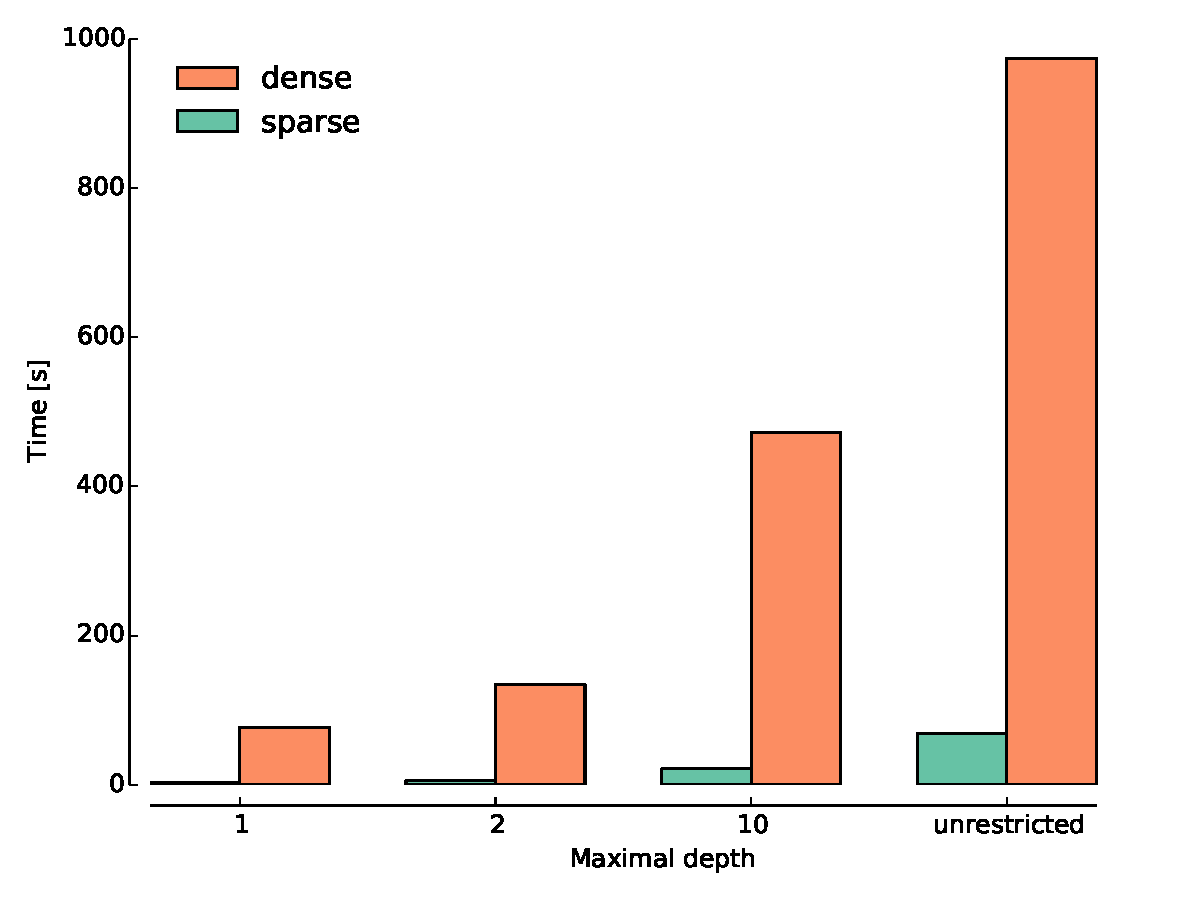
\includegraphics[scale=0.45]{images/depth.pdf}
%\caption{Leveraging the input sparsity significantly speed up decisions
%         tree induction both with shallow and deep trees on the \emph{20 Newsgroups}
%         dataset.}
%\label{fig:depth}
%\end{figure}



\begin{figure}[h]
\centering
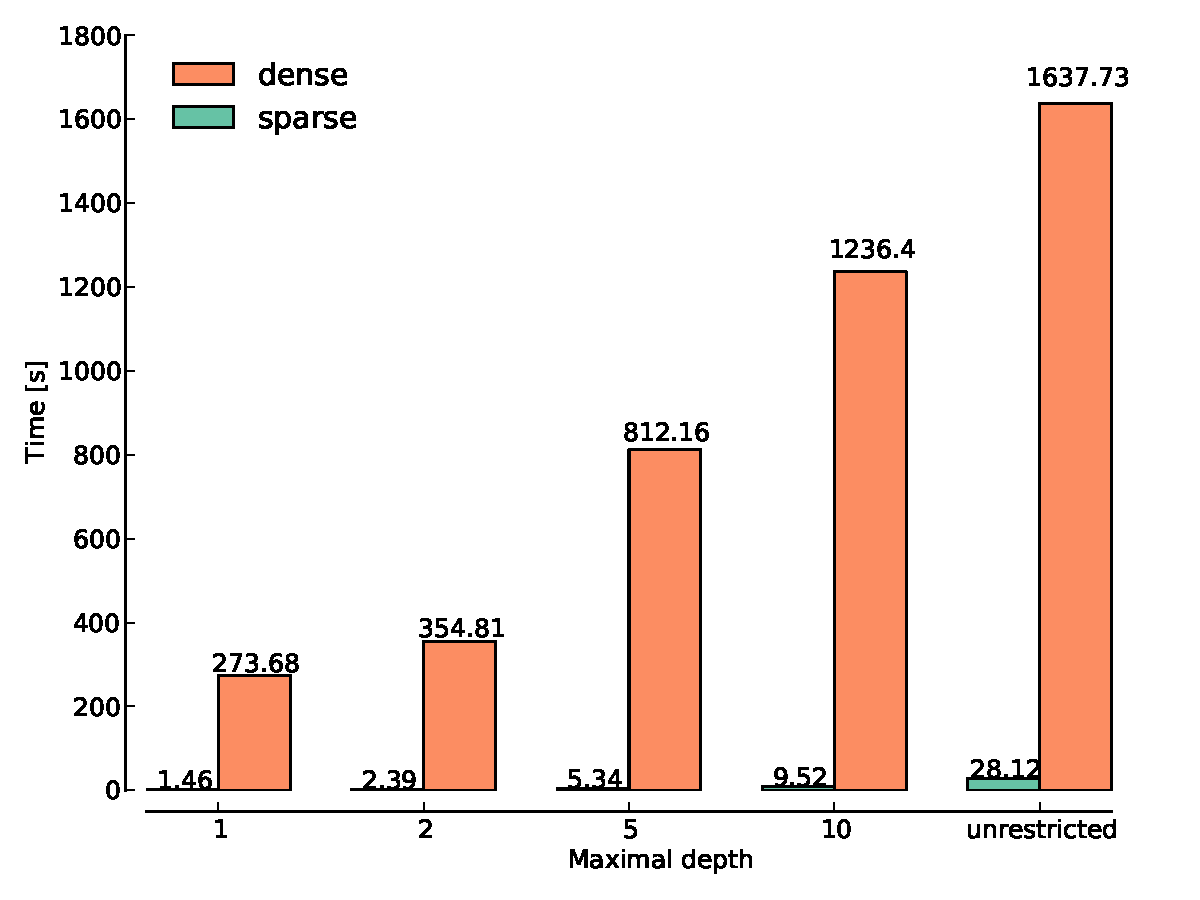
\includegraphics[scale=0.45]{images/20news.pdf}
\caption{Leveraging the input sparsity significantly speed up decisions
         tree induction both with shallow and deep trees on the \emph{20 Newsgroups}
         dataset. Note that the dataset is very sparse (density = 0.001).}
\label{fig:20news}
\end{figure}

\begin{figure}[h]
\centering
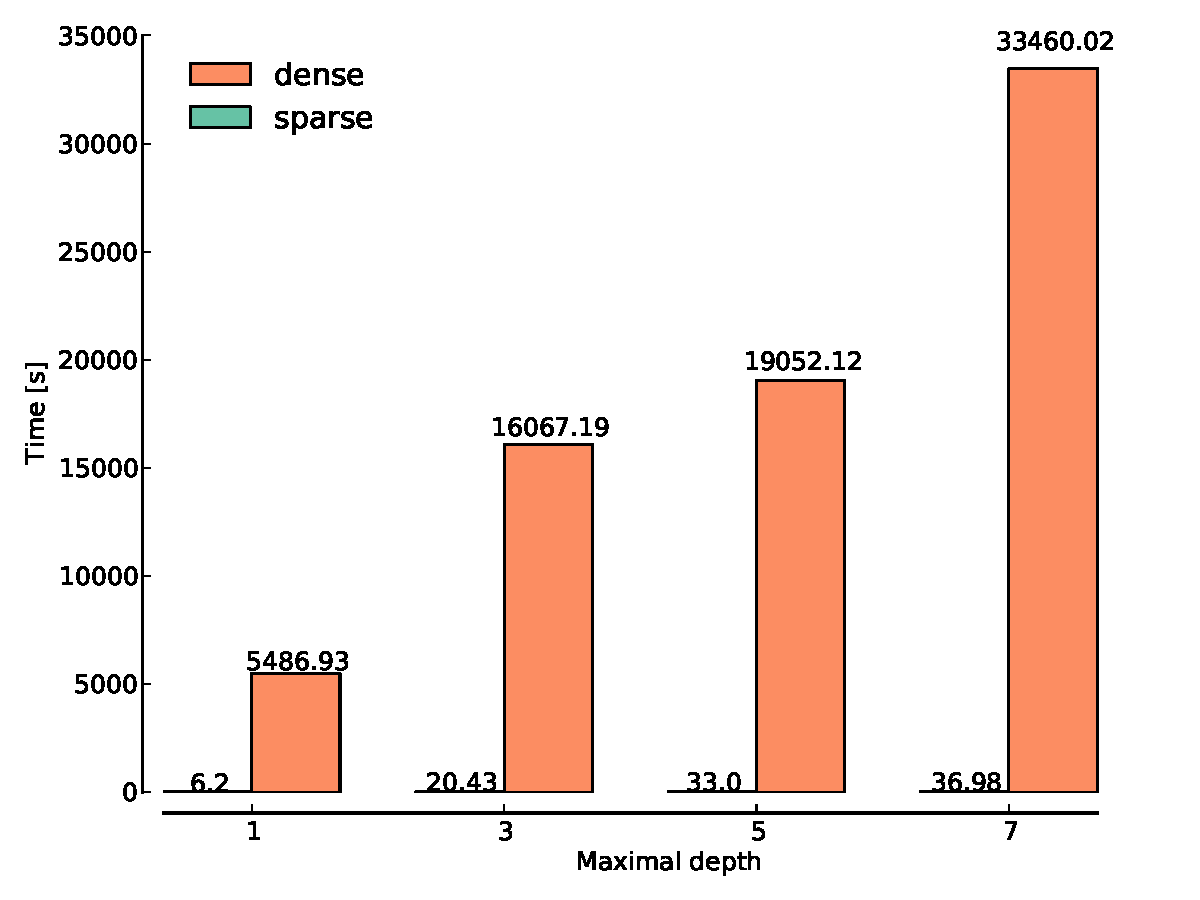
\includegraphics[scale=0.45]{images/cup.pdf}
\caption{Leveraging the input sparsity significantly speed up decisions
         tree induction both with shallow and deep trees on the \emph{cup}
         dataset. Note that the dataset is quite sparse (density = 0.014).}
\label{fig:cup}
\end{figure}



\begin{figure}[h]
\centering
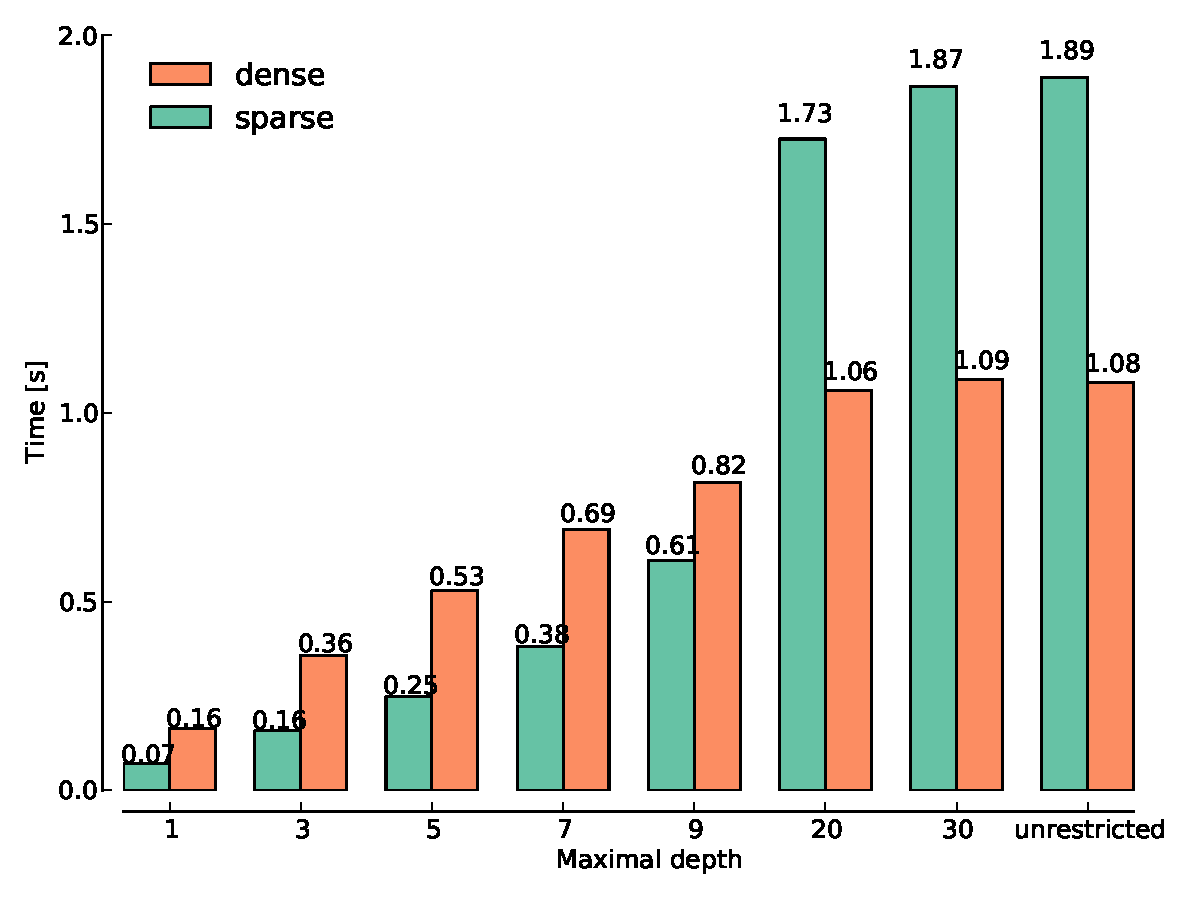
\includegraphics[scale=0.45]{images/adult.pdf}
\caption{Leveraging the input sparsity does not speed up training of deep trees on the \emph{adult}
         dataset. Note that the dataset is quite dense (density = 0.11).}
\label{fig:adult}
\end{figure}


\begin{figure}[h]
\centering
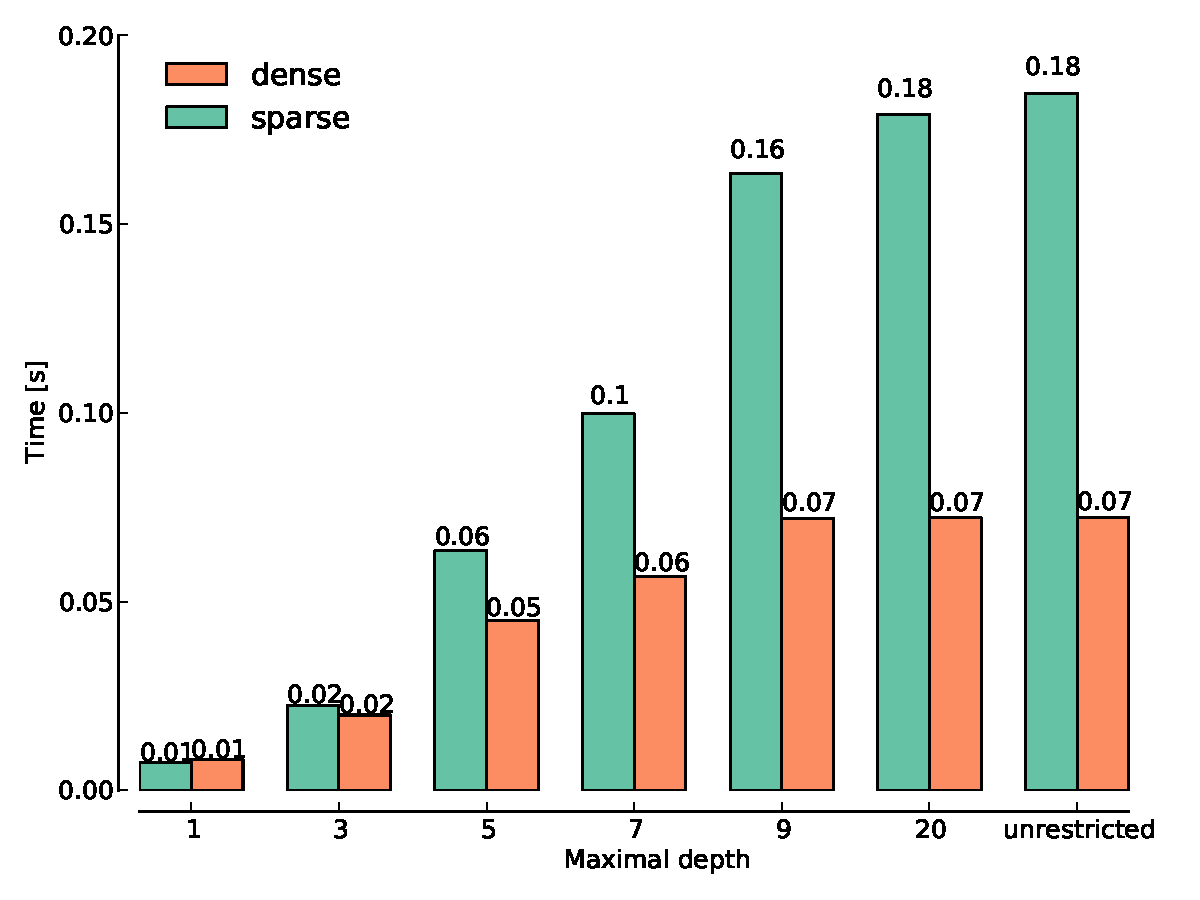
\includegraphics[scale=0.45]{images/tic.pdf}
\caption{Leveraging the input sparsity does not speed up training trees on the \emph{tic}
         dataset. Note that the dataset is very dense (density = 0.44).}
\label{fig:tic}
\end{figure}





\begin{figure}[h]
\centering
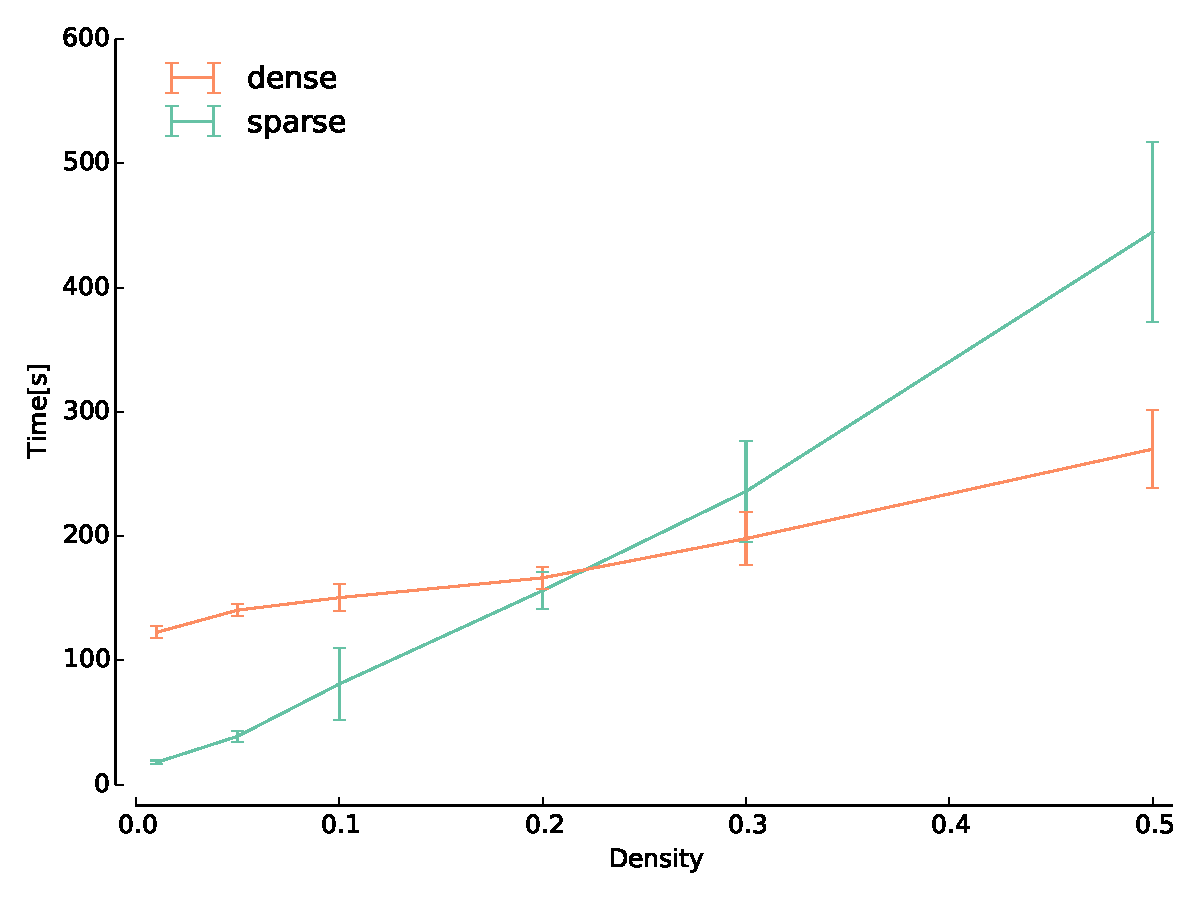
\includegraphics[scale=0.45]{images/density.pdf}
\caption{Significant speed up is achieved by the sparsity-aware decision tree
         algorithm whenever the density is below 0.2 (or sparsity over 0.8).}
\label{fig:density}
\end{figure}
\section{Related Work}
\label{sec:related}

Decision tree learning.
Hastie et al\cite{hastie:book2008} 

Scalable open source implementations: Apache Mahout Spark Mlib

Scalable implementations of other machine learning algorithms such as SVM and Logistic Regression: liblinear

Parallel implementation of trees in Mlib \cite{das:blog2014}

\section{Conclusion}
\label{sec:conclusion}
We proposed a method for building tree-based models with sparse input
support.  Our method takes advantage of input sparsity by avoiding
sorting sample sets of a node along a feature unless they are nonzero
at that feature. This approach speeds up training substantially as
sorting is a costly but essential and ubiquitous component of
tree-based models.

\section{Acknowledgment} % use section* for acknowledgement
Arnaud Joly is a research fellow of the FNRS, Belgium. This work is
partially supported by PASCAL2 and the IUAP DYSCO, initiated by the
Belgian State, Science Policy Office.

%
% The following two commands are all you need in the
% initial runs of your .tex file to
% produce the bibliography for the citations in your paper.
\bibliographystyle{abbrv}
\bibliography{references}  % sigproc.bib is the name of the Bibliography in this case
% You must have a proper ".bib" file
%  and remember to run:
% latex bibtex latex latex
% to resolve all references
%
% ACM needs 'a single self-contained file'!
%
%APPENDICES are optional
\balancecolumns
\end{document}
